\documentclass[12pt]{article}
\usepackage[brazil]{babel}
\usepackage{amsthm}
\usepackage{design_ASC}
\usepackage{pdfpages}
\usepackage{caption}
\usepackage{lipsum}
\usepackage{enumitem, kantlipsum}
\usepackage{indentfirst}
\renewcommand\refname{Referências bibliográficas}
\title{\textbf{Intratabilidade}} %% Assignment Title

\date{}

\author{
André Luís Mendes Fakhoury\\ Eduardo Dias Pennone\\ Gustavo Vinícius Vieira Silva Soares\\ Matheus Steigenberg Populim\\ Thiago Preischadt Pinheiro\\\\
\textsc{SCC0205 - Teoria da Computação e Linguagens Formais}\\
Prof. Diego Raphael Amancio
}

%% %%%%%%%%%%%%%%%%%%%%%%%%%
\begin{document}

\setlength{\droptitle}{-5em}
%% %%%%%%%%%%%%%%%%%%%%%%%%%
\maketitle

\section{Introdução}

\section{Computação eficiente}
\section{Classes P e NP}
\section{Hipóteses P $\neq$ NP}
\section{Reduções em tempo polinomial}

\section{Problemas NP-Difíceis}
\subsection{Exemplos de problemas NP-difíceis}

\begin{trivlist}
\item \textbf{Caixeiro viajante (TSP) - versão de otimização:} dado um grafo $G(V, A)$, encontrar um caminho que visite todas os vértices exatamente uma vez, e que volte ao vértice de origem, de forma a minimizar a distância total (soma das arestas).
\end{trivlist}

\begin{figure}[h!]
    \centering
    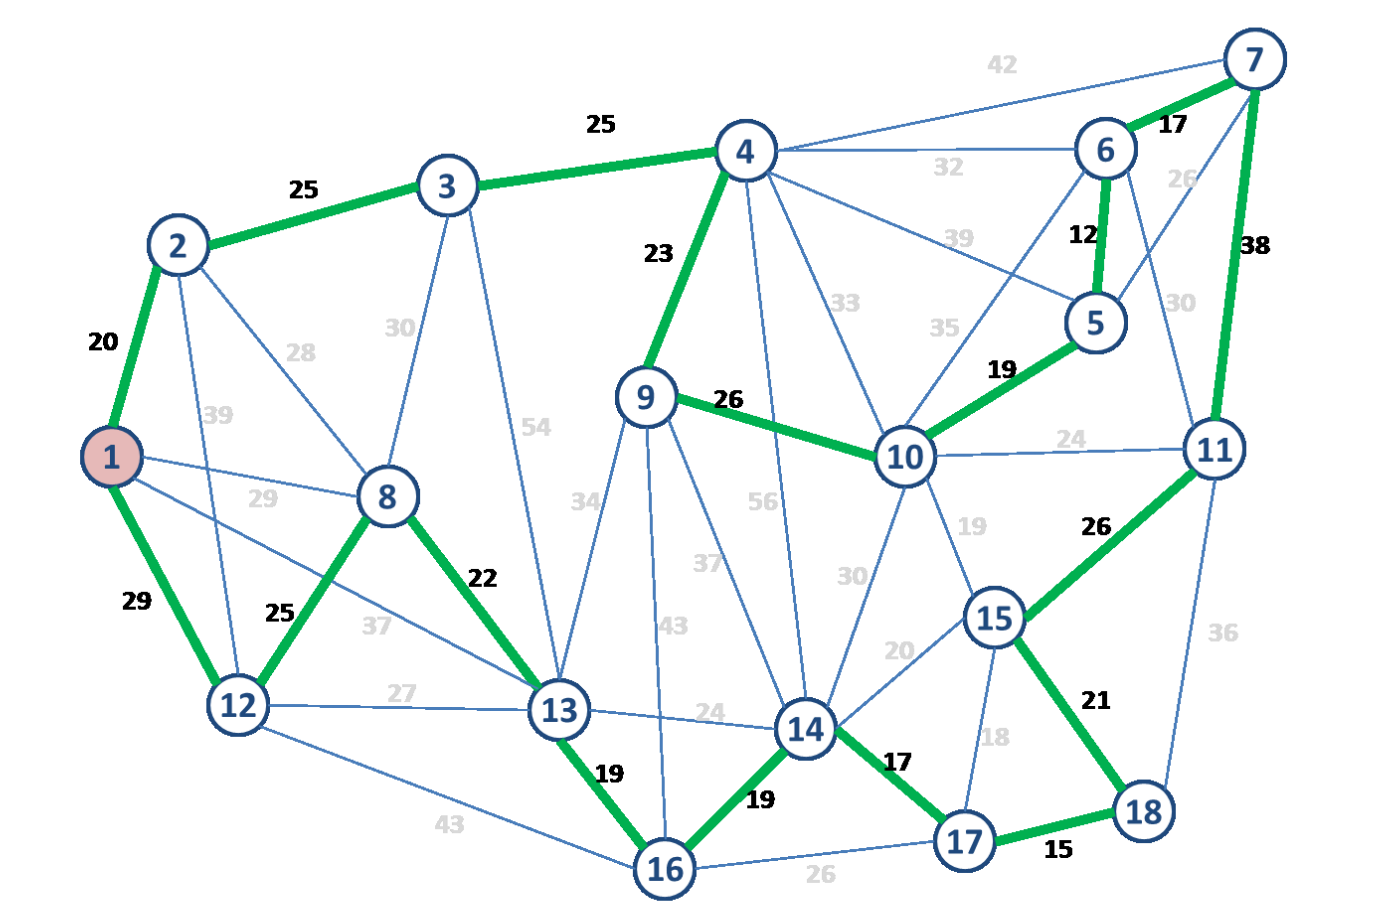
\includegraphics[scale=0.22]{img/tsp.png}
    \captionsetup{labelformat=empty}
    \caption{Exemplo com solução para o caixeiro viajante \cite{valeri2019}}
\end{figure} % arquivo npdificil.tex

\newpage
\newpage

\section{Problemas NP-Completos}

Durante a década de 1970, Stephen Cook e Leonid Levin propuseram, independentemente, um importante avanço na questão de P vs. NP. Eles descobriram alguns problemas pertencentes a NP em que a complexidade individual está relacionada com toda a classe - e, caso um algoritmo em tempo polinomial exista para algum destes problemas em específico, então todos os problemas em NP também podem ser resolvidos em tempo polinomial. Estes \textit{problemas em específico} são denotados \textbf{NP-completos}. Por esta importante característica, os estudos neste campo podem ser focados nos problemas \textit{NP-completos}.

\begin{definition}{(NP-Completo)}
Uma linguagem $B$ é dita \textit{NP-completa} caso satisfaça estas duas características:
\begin{enumerate}[nosep]
    \item $B$ está em $NP$;
    \item Todo $A$ em $NP$ é redutível em tempo polinomial para $B$;
\end{enumerate}
\end{definition}

Também pode-se utilizar a classe \textit{NP-difícil} para definir os problemas \textit{NP-completos}: um problema \textit{NP-completo} é \textit{NP-difícil} e está em \textit{NP}. Outro teorema que será útil para definir se uma linguagem $C$ é \textit{NP-completa} é a seguinte:

\begin{theorem}{(NP-Completo)}
Se $B$ é \textit{NP-completo} e $B \leq_p C$ ($B$ é redutível em tempo polinomial para $C$) para $C$ em $NP$, então $C$ é \textit{NP-completo}.
\end{theorem}

Assim, ao se conhecer um problema \textit{NP-completo}, pode-se utilizar o conceito de \textit{redução em tempo polinomial} para mostrar que outros problemas são \textit{NP-completos}. A prova deste teorema é a seguinte: já se sabe que $C$ está em $NP$, então, pela definição, basta provar que todo $A$ em $NP$ é redutível em tempo polinomial para $C$. Como $B$ é \textit{NP-completo}, todo $A$ é redutível em tempo polinomial para $B$. Como todo $A$ é redutível para $B$ e $B$ é redutível para $C$, tem-se que todo $A$ também pode ser redutível para $C$.

Ainda assim, é necessário um passo inicial: provar que um problema é \textit{NP-completo} sem serem conhecidos outros problemas \textit{NP-completos} (em que se poderia utilizar redução polinomial para facilitar a prova). O primeiro problema demonstrado NP-completo foi o problema SAT (satisfatibilidade booleana), por Cook e Levin, que será discutido no próximo tópico.

\subsection{Exemplos de problemas NP-completos}

Serão aqui discutidos alguns exemplos de problemas definidos como \textit{NP-completos}.


\begin{trivlist}
\item \textbf{Satisfatibilidade booleana (SAT):} verificar se existe uma valoração para as variáveis que compõe uma fórmula booleana, de forma que esta tenha saída verdadeira.
\end{trivlist}

O SAT é, historicamente, o primeiro problema provado como \textit{NP-completo}. Outro ponto interessante é que este problema é \textit{auto-redutível}, ou seja, o algoritmo que resolve o problema (e verifica se existe tal composição de valores para variáveis) também consegue encontrar a atribuição de variáveis satisfatórias. O teorema que afirma que o SAT é NP-completo é chamado \textbf{teorema de Cook-Levin}, e, devido à sua complexidade, sua prova não será abordada neste trabalho.

\begin{trivlist}
\item \textbf{3SAT:} problema SAT com expressões na forma normal conjuntiva, e cada cláusula contém exatamente três variáveis.
\end{trivlist}

Pode-se provar que o 3SAT é NP-Completo a partir do problema SAT original: é possível deduzir, em tempo polinomial, qualquer caso de SAT para um caso equivalente em 3SAT. Além disso, pode-se afirmar que 3SAT é NP, pois, dada uma coleção de cláusulas e uma valoração para as variáveis, é possível verificar em tempo polinomial se estas cláusulas são satisfeitas (basta percorrer as cláusulas e atribuir os valores das variáveis, verificando se a resposta é verdadeira).

Para fazer esta dedução de caso SAT para 3SAT, a expressão é primeiramente denotada na forma normal conjuntiva (conjunção de disjunções). Com a expressão nesta forma, é possível reduzir cláusulas com mais de três termos em duas ou mais cláusulas de 3 termos: por exemplo, a disjunção $(A \lor B \lor C \lor D)$ pode ser reduzida introduzindo uma nova variável $E$ (sem importância para a expressão original) para $(A \lor B \lor E) \wedge (\neg E \lor C \lor D)$.

Outro problema de satisfatibilidade é o problema 2SAT. Este, caso as fórmulas estiverem restringidas à forma normal conjuntiva (conjunção de disjunções), pode ser resolvido em tempo polinomial (por exemplo, utilizando-se componentes fortemente conexas).

\begin{trivlist}
\item \textbf{Clique:} dado um grafo $G(V, A)$ e um inteiro $k$, encontrar se existe um subgrafo de $k$ ou mais vértices, em que todos nós dois a dois são conectados por uma arestas - ou seja, se $G$ possui um conjunto de $k$ nós mutualmente adjacentes.
\end{trivlist}

Precisa-se provar, inicialmente, que o clique é NP: é possível construir um verificador que recebe um grafo $G(V, A)$, um inteiro $k$ e um conjunto $S$. Será feita a verificação se $S$ possui tamanho maior ou igual a $k$, e, então, verificar se para cada par de vértices $(u, v) \in S$ existe uma aresta $(u, v) \in A$. Esta verificação pode ser feita em $\mathcal{O}(|S|^2)$.

Agora, prova-se que o clique é \textit{NP-difícil}. Para isso, pode-se mostrar que existe uma redução do problema \textit{3SAT} para o problema \textit{clique}. Será feita a construção de uma função que recebe qualquer instância do 3SAT e retorna uma instância de Clique, que é verdadeira se e somente se a instância do 3SAT for verdadeira. Dado uma expressão booleana (na forma 3SAT) com cláusulas $c_1, \dots, c_m$ e variáveis $x_1, \dots, x_n$, pode-se construir um grafo $G(V, A)$ com $|V| = 3m$ da seguinte forma:

\begin{itemize}
    \item Para cada cláusula $c_j = (l_1^j \lor l_2^j \lor l_3^j)$ constrói-se 3 vértices $l_1^j, l_2^j, l_3^j$
    \item Para cada par $l_i^j, l_k^t$ é adicionada uma aresta entre eles se e somente se:
    \begin{itemize}
        \item As cláusulas $j$ e $t$ são diferentes;
        \item $l_i^j \neq \neg l_k^t$ (são consistentes)
    \end{itemize}
\end{itemize}

Como cada um dos três vértices de uma mesma cláusula não estão ligados entre si, cada clique contém, no máximo, um deles. Ou seja, o tamanho máximo possível para um clique é $m$. E, um clique de tamanho $m$ existe se e somente se o 3SAT for satisfatível, pelos seguintes itens \cite{peng2016}:

\begin{itemize}
    \item Caso exista um clique, os vértices envolvidos no clique não possuem conflitos com outros (pois serão consistentes). Assim, pode-se designar os valores para cada variável. Como tem-se apenas um literal por cláusula, cada cláusula terá um literal satisfeito, tornando isso uma valoração satisfatível.
    \item Caso tenha uma valoração satisfatível para as variáveis, cada cláusula possui um literal satisfeito, e, como nenhum destes literais tem conflito com nenhum outro, existem arestas entre eles, dando o clique de tamanho $m$.
\end{itemize}

\begin{trivlist}
\item \textbf{Cobertura de vértices (\textit{Vertex-Cover}) - versão de decisão:} dado um grafo $G(V, A)$ e um inteiro $k$, encontrar se existe um subconjunto de vértices $V'$ de tamanho $k$ tal que toda aresta em $A$ esteja conectada em no mínimo um vértice em $V'$.
\end{trivlist}

Para se provar que este problema é NP-Completo, primeiramente, mostra-se que este problema é NP. Dado um subconjunto $V'$, pode-se verificar com complexidade polinomial se este é um subconjunto correto (basta percorrer por todas as arestas e verificar se algum de seus vértices pertence ao conjunto $V'$), logo, é NP. Após isso, pode-se também mostrar que o problema do Clique pode ser reduzido em tempo polinomial para um exemplo de problema de cobertura de vértices - esta prova não será demonstrada neste trabalho.

\begin{trivlist}
\item \textbf{Circuito hamiltoniano (HAMPATH):} verifica se existe um circuito hamiltoniano entre $s, t$ em um grafo $G$.
\end{trivlist}

O problema do circuito hamiltoniano consiste em, dado um grafo $G(V, A)$ e dois vértices $s, t \in V$, existe um caminho de $s$ até $t$ que passa por todos os vértices $\in V$ exatamente uma vez. Para provar este teorema, primeiramente precisa-se provar que ele é NP. Isto pode ser verificado pois, dado um circuito $C$, pode-se facilmente verificar se este é um circuito válido com complexidade polinomial $\mathcal{O}(|V| + |A|)$. Agora, resta provar que existe um problema NP-completo que possua uma redução em tempo polinomial para o \textit{HAMPATH}. Pode-se escolher, por exemplo, o 3SAT para realizar esta prova - que também não será demonstrada neste trabalho.

\begin{trivlist}
\item \textbf{Caixeiro viajante (TSP) - versão de decisão:} dados um grafo $G(V, A)$ e uma distância $L$, retornar se existe um ciclo (que visite todos os vértices exatamente uma vez) com distância total no máximo $L$.
\end{trivlist}

Embora a variação de otimização do problema seja ``apenas'' considerada \textit{NP-difícil} (como visto anteriormente), pode-se definir a versão de decisão do TSP como \textit{NP-completa}. Para provar que esta variação é NP, dado um grafo $G(V, A)$, um inteiro $L$ e um ciclo $c$, pode-se verificar se o ciclo $c$ de fato é um ciclo válido neste grafo, e se a soma de suas arestas não ultrapassa o limite $L$ - esta verificação é feita polinomialmente, podendo ser feita com complexidade $\mathcal{O}(|c|)$.

Para provar que esta variação é NP-difícil, pode-se construir uma redução em tempo polinomial de outro problema NP-completo, o \textit{problema do ciclo hamiltoniano} - ou seja, mostrar que $\text{HamCycle} \leq_p \text{TSP}$. Para isso, seleciona-se que qualquer instância $G(V, A)$ do ciclo hamiltoniano. Objetiva-se montar uma instância do TSP, em que o grafo $G'(V', A')$ do TSP é montado da seguinte forma:

\begin{itemize}
    \item $V' = V$ (utiliza-se os mesmos vértices)
    \item $E' = \{(u, v) : u, v \in V \And u \neq v\}$
\end{itemize}

E o custo de cada aresta $e$ em $E'$ é calculado da seguinte forma:

$$
c(e) = 
\begin{cases}
\text{0, se } e \in E\\
\text{1, se } e \notin E
\end{cases}$$

Agora, suponha que um ciclo hamiltoniano $h$ exista em $G$. O custo de cada aresta de $h$ em $G'$ é $0$, visto que todas as arestas estão no conjunto $E$. Desta forma, $h$ tem custo 0 em $G'$. De maneira análoga, assume-se que $G'$ tem um circuito $h'$ de custo no máximo $0$ - desta forma, as arestas em $E'$ escolhidas tem todas custo $0$. Isto significa que todas as arestas escolhidas em $h'$ também pertencem ao conjunto $E$. Assim, pôde-se concluir uma redução (em tempo polinomial) do problema do ciclo hamiltoniano para esta versão do TSP, provando-se que esta variação do TSP é NP-difícil.

\begin{trivlist}
\item \textbf{Outros exemplos}
\end{trivlist}

Também existem vários outros problemas clássicos \textit{NP-completos} (ou com variações que são), como, por exemplo, coloração completa em grafos (número acromático), conjunto independente máximo, \textit{Steiner tree} (árvore geradora mínima para um subconjunto de vértices de um grafo), \textit{bin packing}, soma de subconjuntos e batalha naval. Existem diversos livros e artigos listando mais diversos problemas assim classificados - um dos mais importantes artigos deste tema foi feito por Richard Karp \cite{karp1972}. % arquivo npcompleto.tex


%%%%%%%%%%%%%%%%%%%%%%%%%%%%%%%%%%%%%%%%%%%%%%

\section{Conclusão}

A teoria de NP-completude garante diversas formas de provar que determinados problemas são "tão difíceis" quanto vários outros estudados. Por exemplo, se certa pessoa está tentando resolver um problema, e este problema pode ser provado como \textit{NP-completo}, ela pode ficar mais tranquila caso não consiga achar uma solução (pois, até hoje, esta solução ainda não foi encontrada). Por isso, o estudo de complexidade e intratabilidade é de suma importância no estudo de computação, e a separação dos problemas em classes de acordo com suas possibilidades de serem resolvidos em tempo polinomial ou não (dilemas P vs. NP) é muito interessante.

\nocite{*}
\bibliographystyle{plain} % We choose the "plain" reference style
\bibliography{refs} % Entries are in the "refs.bib" file

% \begin{thebibliography}{9}





% \end{thebibliography}

\end{document}